\documentclass[a4paper]{scrartcl}
\usepackage[utf8]{inputenc}
\usepackage[english]{babel}
\usepackage{graphicx}
\usepackage{lastpage}
\usepackage{pgf}
\usepackage{wrapfig}
\usepackage{fancyvrb}
\usepackage{fancyhdr}
\usepackage{hyperref}
\pagestyle{fancy}

\catcode`\_=\active
\protected\def_#1_{\textit{#1}}

% Create header and footer
\headheight 27pt
\pagestyle{fancyplain}
\lhead{\footnotesize{Distributed Systems - Advanced, ID2203}}
\chead{\footnotesize{Project}}
\rhead{}
\lfoot{}
\cfoot{\thepage}
\rfoot{}

% Create title page
\title{Distributed Key-Value Store}
\subtitle{Distributed Systems - Advanced, ID2203}
\author{Bernardo Gonzalez Riede \& Vinit Kumar Verma}
\date{\today}

\begin{document}

\maketitle

%Introduction
\section{Introduction}

\subsection{Goals}
The overall goal is to have a distributed, partitioned and in-memory key-value store. 
While not explicitly mentioned, the abstractions used throughout the course and the book are fundamental for planning and reasoning about the system development. Imbuing them and relying on underneath abstractions might reduce complexity considerably while working on a certain module/layer. 

\subsection{Requirements}
The following points had to be covered:
\begin{itemize}
\item Linearizable operation semantics
\item Development of test scenarios
\item _GET_, _PUT_ and _CAS_ operations
\end{itemize}

%Reasoning
\section{Reasoning \& Motivation}

\subsection{Distributed system model assumption}

The model assumed is the fail-noisy one.
The following sections will motivate the decision made.

\subsubsection{Process/crash abstraction}
Byzantine failures won’t be covered. While a reality, it introduces a significant amount of complexity. The probability of a malicious failure during the development is low enough to be negligible. Arbitrary faults in the form of corrupted messages will be prevented by using TCP/IP. Moreover, being a memory key value store one could argue about the usage of ECC buffered RAM which corrects corrupt memory, which itself is already an unlikely one-time failure.
If a node crashes, it won’t be restarted itself which makes omissions the only reason for using the crash-recovery model. Omissions may incur in the following way:

\begin{itemize}
\item A node is overloaded
\item A message is lost in transit
\item Network partition
\end{itemize}

A node overload can be prevented by vertical scaling while the perfect link abstraction assures exactly-once delivery.
For this project it’s feasible to assume that a high amount of crashes is unlikely, meaning a majority of correct nodes exists. Therefore the crash-stop model will be used.


\subsubsection{Communication assumptions}
Being the abstraction mostly used during the course and guaranteeing exactly-once delivery, perfect links will be used for communication.

\subsubsection{Timing assumptions}
Running the nodes on the same machine can allow for a synchronous system, although a growing key value store might pose a problem in terms of computation time.
On the other hand, an asynchronous system is very weak and there exists a stronger model with real world value.
The partially asynchronous system is the model of the internet and the one used in the project.



\subsection{Design choices}


\subsubsection{Bootstrapping}
Bootstrapping is the only weakness of the system.
During bootstrapping the bootstrap servers poses a single point of failure.
It reads the replication degree and the amount of partions wanted from a configuration file and waits until enough nodes have checked in to be able to form the distibuted \& partitioned KV-store.
It sends the generated lookup table to all nodes.

Each node then extracts the list of nodes of its own partitions to start the _SequencePaxos_, which in turn starts the _BLE_, for the partition.
Moreover, Ev.P is used to monitor all nodes in the system as to only provide a newly connected client only with a not suspected node as entry point

\subsubsection{Partitioning}
Partitioning is done automatically through the bootstrapping node which divides the total number space an _integer_ can have to create even partitions. 
This decision is the result of the provided code base which includes a _String.toHash()_ method returning an _integer_.

\subsubsection{Replication}
A shared memory abstraction is too weak to provide a compare and swap operation, therefore motivating the need of implementing a replicated state machine.
This was done using the _SequencePaxos_ algorithm from the course which is a leader-based sequence consensus.

\subsubsection{Resilience}
Google has mentioned that  _f = 3_ is a good value, providing enough resilience for a real world scenarion.
Being a small scale project for learning purposes the decision fell upon _f = 1_ for development and test.
Nonetheless the value can be changed in the configuration file.

\subsubsection{Client}
The client only needs to know one correct process to be able to use the service.
It connects to one server, which in turn will return a list of not suspected nodes at the time of connecting.
The client may then go through the list or keep using the same node until an operation failes.




%Implementation
\section{Implementation}

\subsection{Codebase}
The scala codebase was used as a head start for the implementation.
Figure \ref{fig:initial} shows the component diagram of the provided scala code base. 

\begin{figure}[h!]
  \begin{center}
    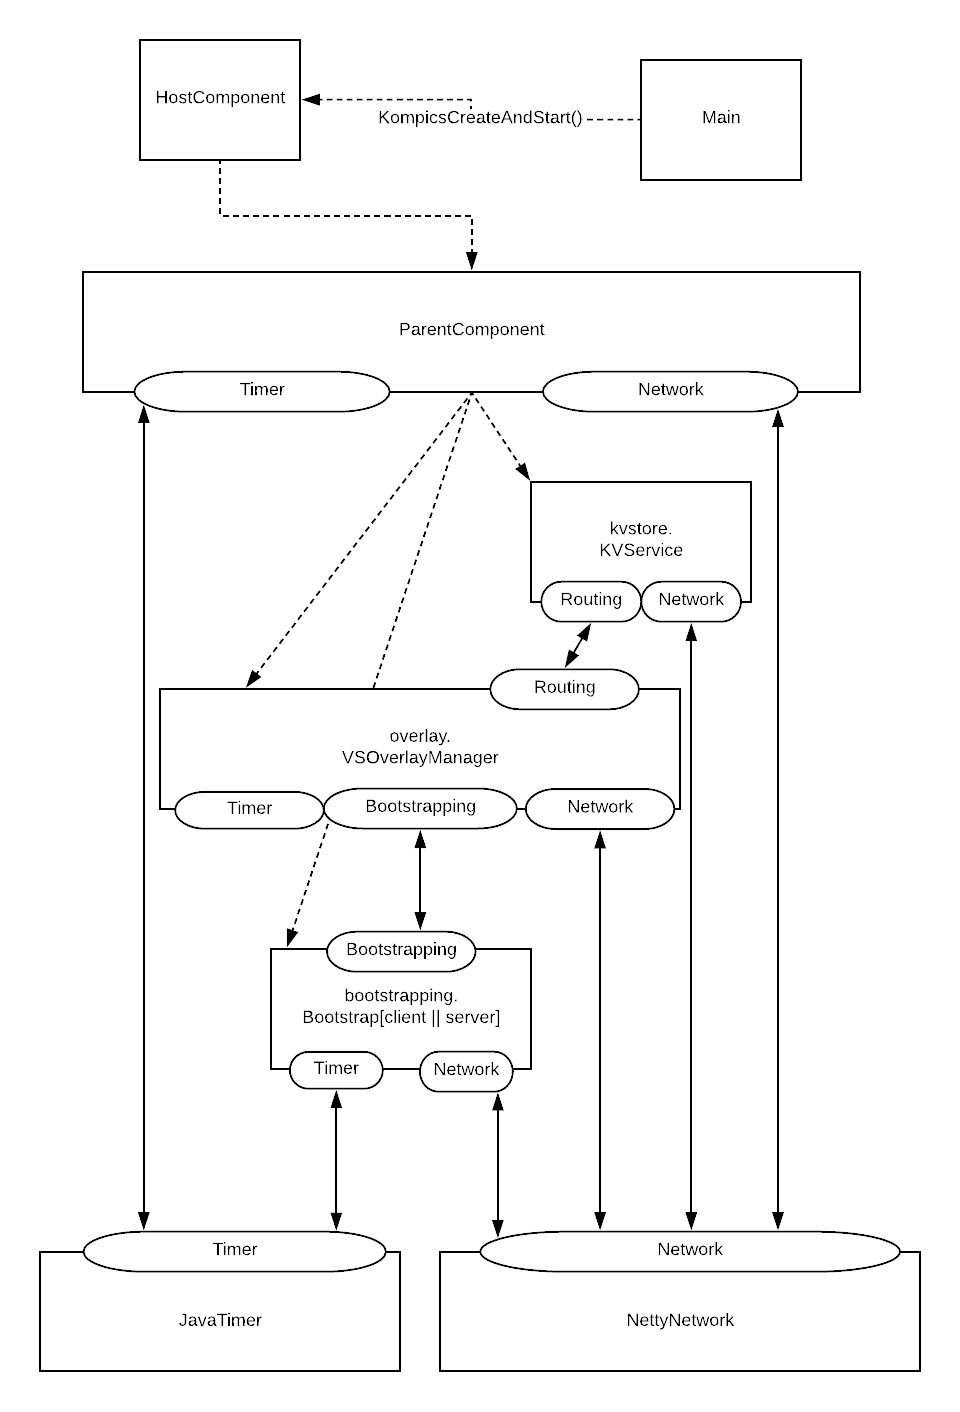
\includegraphics[scale=0.4]{Initial.png}
    \caption{Component Hierarchy of the code template}
    \label{fig:initial}
  \end{center}
\end{figure}

\subsection{Added code}
Figure \ref{fig:modified} shows only the added components and affected components from the template except _Timer_ and _Network_ which should be clear.
Furthermore the diagram shows the component using the network component although the code from the exercises rely on a _PerfectLink_ in the code. 
Being only a wrapper  for the network component the diagram shows no diferrence to the real world behaviour.
This is thanks to the underlying usage of TCP which provides session based FIFO perfect links.

\begin{figure}[h!]
  \begin{center}
    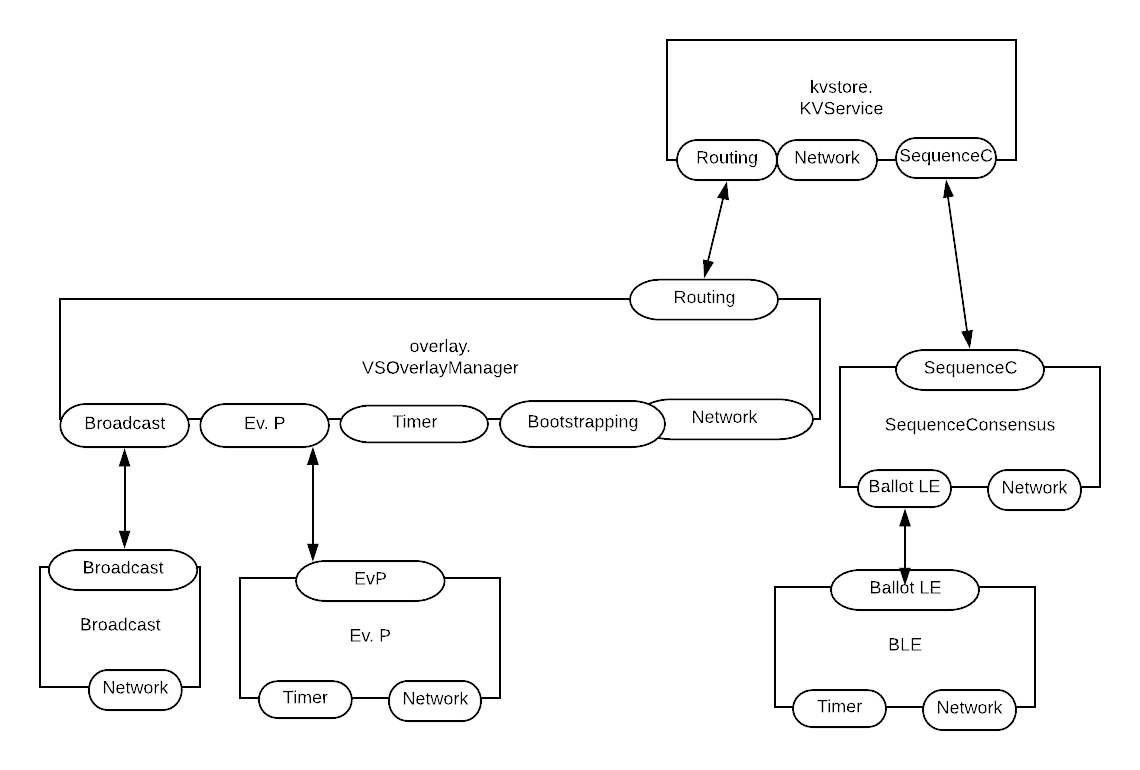
\includegraphics[scale=0.4]{Modified.png}
    \caption{Purview of the added components}
    \label{fig:modified}
  \end{center}
\end{figure}

The components from the exercises where copied for the most part, but refined in some ways to fit the use case.
Especially regarding the starting of _Ev.P_ and _BLE_ since the nodes don't know the other nodes in their replication group until bootstrapping is finished which required the introduction of a _Monitor_ and _SetTopology_ events.

\subsubsection{Configuration file}
The configuration file was extended to hold more values related to the project:
\begin{itemize}
\item _replicationDegree_ = amount of nodes in a replication group
\item _partitions_ = amount of partitions to create
\item _prefillStore_ = how many values to prefill the KV-store
\end{itemize}

\subsection{Operation Invocation}
As the saying goes: "A picture says more than a thousand words.", \ref{fig:invocation} shows the event flow from an operation invocation by a client until being included in the list of commands to agree upon.

\begin{figure}[h!]
  \begin{center}
    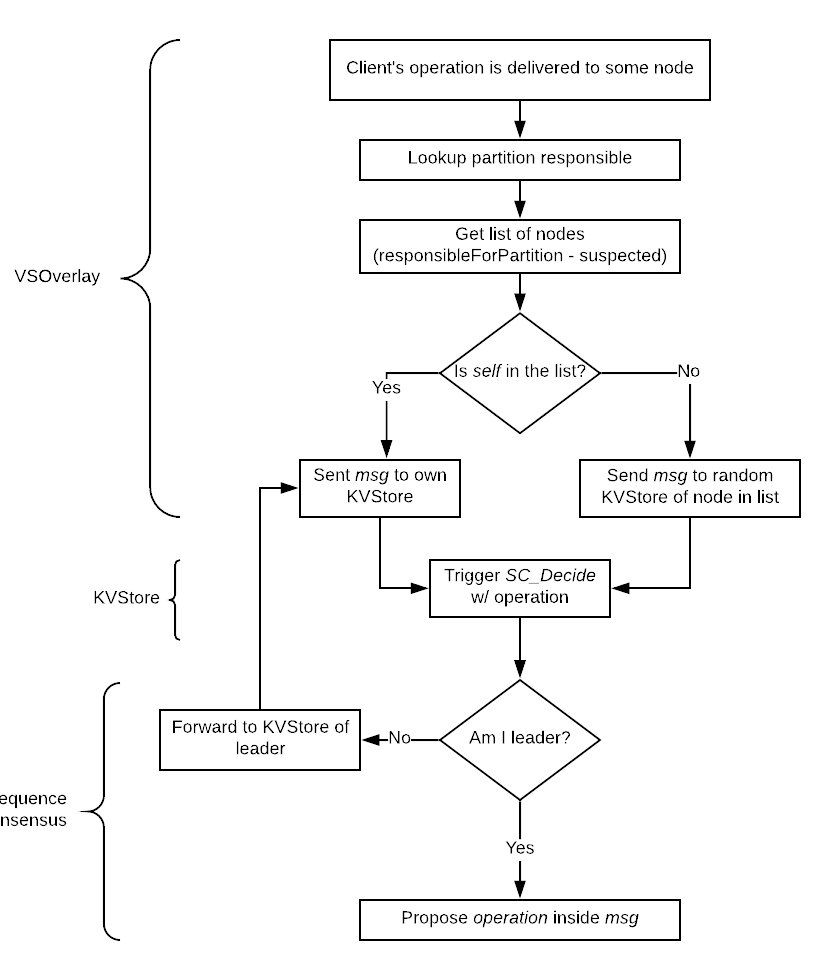
\includegraphics[scale=0.4]{OperationFlowInvocation.png}
    \caption{Flowchart of operation invocation}
    \label{fig:invocation}
  \end{center}
\end{figure}

\subsection{Operation  reply}
Through the guarantees of the sequence consensus the KVstore safely executes an operation after a _SCDecide_ event.
For the client to know be informed about the result, i.e. the reply to the invocation, several approaches exists.
\begin{itemize}
	\item Have the first receptor inside the responsible partition save the UUID + source IP of the operation. 
	This allows to let only this node send a reply.
	\item Have the leader send a reply since there will always be a leader once established unless _f \textgreater resilience_ .
	\item Have all nodes in the partition send a reply
\end{itemize}
The first case allows for an omission of the reply should the receptor crash before sending the reply message although the operation might still be executed by the others.

While the second case has the least amount of messages, the last option was implemented. 
The client already has the functionality to ignore replies which it isn't waiting for.
Moreover, the client removes  the pending entry when receiving a reply, thus ignoring duplicate replies which can be identified thanks to the UUID.
Furthermore, it allows for testing cases to count the amount of replies received and comparing the results.
Inconsistencies in the RSM or slow nodes can be detected by comparing the inconming results.


%Testing
\section{Testing}
Testing was done using the kompics simulator library and based mostly on the provided example.

\subsection{Operations}
The simulations save the OpCodes from the _Operation_ class to determine what happened and to be able to differentiate between a value not found or, in the case of CAS, the referenceValue being incorrect. For this an additional OpCode has been incorporated.

\subsubsection{Preloaded KV - GET}
The kv store is filled on  startup with a pair _(test<i>, value<i>)_ for 0 \textless i \textless n, _n_ being a valued defined in the configuration file.
The test tries to retrieve the prefilled values from the KV-Store

\subsubsection{PUT \& CAS}
The test for these include 3 different ways of trying them, especially the compare-and-swap one.
PUT has no individual test, given it being the operation least likely to fail.  Besides not being implemented, it can only fail by the responsible replication group being unavailable.
CAS is tested in three different ways:
\begin{itemize}
\item Fail by not finding the key 
\item Fail by having an incorrect referenceValue
\item Use PUT to insert certain values, afterwards expecting a successful CAS with the newly inserted value
\end{itemize}

\subsection{Replication}
The replication test consist of two runs.

First, a system of one partition and three nodes is created. 
Afterwards the expected leader is killed and after some waiting the client tries to execute some GET operations.
It is known that the bootstrap server will become leader through BLE while in a stable/legitimate state.
Because there continues to exist a majority quorum, sequence consensus will advance as long as no other node crashes.

The second run starts similar but kills two (out of three) nodes instead.
The expected outcome is for the client to timeout the operation since there is no quorum and the sequence consensus won't proceed deciding on commands.

\subsection{Linearizability}
First and foremost, Linearizartion _LIN_ is compositional, i.e. if it is valid for one register it holds for the whole system.
Additionally, for LIN to hold for each execution, a legal history S has to exists, such that
\begin{itemize}
\item S is equivalent to T \textbar xr
\item S preserves the order of non-overlapping operations in said T
\end{itemize}


To prove this, 3 test cases were created and testet:
\begin{enumerate}
\item Ow \textless Ow - using first a PUT and a CAS afterwards using the newly added value from PUT
\item Or \textless OW - using a GET to retrieve a value and a CAS with the referenceValue again afterwards
\item Ow \textless Or - using a PUT and a Get afterwards which needs to retrieve the value written
\end{enumerate}

The ability to use CAS helped to establish a connection between consequent writes to see that indeed they are executed sequentially if non overlapping.

%Conclusion
\section{Conclusion}
Devevloping the application seemed overwhelming at the beginning of the course. 
The most difficult part was to start, but after having looked at some of the content of the course it helped to understand the problem.

The second obstacle was to prove linearizability which resulted arduous.


\end{document}
